\section{实验结果}
\label{sec:experimental-results}

本文开展了两类测试：一类用于验证算法是否能够正确完成立体校正，另一类用于检验直接从校正图像进行三维重建时，重建精度是否会降低。

\paragraph{正确性。}
测试同时使用了合成数据和真实数据。每组合成数据由一组 3D 点云和一对 PPM 构成。受篇幅限制，本文只报告两个示例。图~\ref{fig:fig3} 展示了一个近似校正的双目系统所得到的原始图像和校正图像：相机平移为
\[
-\left[100\;2\;3\right] \,\mathrm{mm},
\]
旋转角分别为 $\mathrm{roll}=1.5^\circ$、$\mathrm{pitch}=2^\circ$ 和 $\mathrm{yaw}=1^\circ$。图~\ref{fig:fig4} 展示了更一般几何结构下的相同结果：相机平移为
\[
-\left[100\;20\;30\right] \,\mathrm{mm},
\]
旋转角分别为 $\mathrm{roll}=19^\circ$、$\mathrm{pitch}=32^\circ$ 和 $\mathrm{yaw}=5^\circ$。

\begin{figure}[htbp]
  \centering
  \IfFileExists{figures/fig3.png}{%
    \includegraphics[width=0.96\linewidth]{figures/fig3.png}%
  }{%
    \IfFileExists{task1/figures/fig3.png}{%
      \includegraphics[width=0.96\linewidth]{task1/figures/fig3.png}%
    }{%
      \fbox{\parbox[c][3.0cm][c]{0.72\linewidth}{\centering 图 3 原图待提取\\\small 路径：figures/fig3.png}}%
    }%
  }
  \caption{近似校正的合成双目图像对（上）及校正后的图像对（下）。图中给出了两幅图像中以圆圈标记的点所对应的对极线。}
  \label{fig:fig3}
\end{figure}

\begin{figure}[htbp]
  \centering
  \IfFileExists{figures/fig4.png}{%
    \includegraphics[width=0.96\linewidth]{figures/fig4.png}%
  }{%
    \IfFileExists{task1/figures/fig4.png}{%
      \includegraphics[width=0.96\linewidth]{task1/figures/fig4.png}%
    }{%
      \fbox{\parbox[c][3.0cm][c]{0.72\linewidth}{\centering 图 4 原图待提取\\\small 路径：figures/fig4.png}}%
    }%
  }
  \caption{一般几何结构下的合成双目图像对（上）及校正后的图像对（下）。图中给出了两幅图像中以圆圈标记的点所对应的对极线。}
  \label{fig:fig4}
\end{figure}

真实数据实验使用了经过标定的双目图像对，数据由 INRIA-Syntim 提供。图~\ref{fig:fig5} 给出了近似校正的双目系统的结果，图~\ref{fig:fig6} 给出了更一般双目几何结构的结果。校正图像的像素坐标并不受限于图像平面中的某个特定区域；为将两幅图像移到平面中合适的区域，对两幅图像均施加了一个任意平移。随后，将输出图像裁剪为与输入图像相同的尺寸。在 ``Sport'' 双目图像对中（图像尺寸为 $768\times576$），我们从以下相机矩阵开始：

\[
P_{o1}=\left[\begin{array}{rrrr}
9.765\cdot10^{2} & 5.382\cdot10^{1} & -2.398\cdot10^{2} & 3.875\cdot10^{5}\\
9.849\cdot10^{1} & 9.333\cdot10^{2} & 1.574\cdot10^{2} & 2.428\cdot10^{5}\\
5.790\cdot10^{-1} & 1.108\cdot10^{-1} & 8.077\cdot10^{-1} & 1.118\cdot10^{3}
\end{array}\right].
\]

\[
P_{o2}=\left[\begin{array}{rrrr}
9.767\cdot10^{2} & 5.376\cdot10^{1} & -2.400\cdot10^{2} & 4.003\cdot10^{4}\\
9.868\cdot10^{1} & 9.310\cdot10^{2} & 1.567\cdot10^{2} & 2.517\cdot10^{5}\\
5.766\cdot10^{-1} & 1.141\cdot10^{-1} & 8.089\cdot10^{-1} & 1.174\cdot10^{3}
\end{array}\right].
\]

\begin{figure}[htbp]
  \centering
  \IfFileExists{figures/fig5.png}{%
    \includegraphics[width=0.96\linewidth]{figures/fig5.png}%
  }{%
    \IfFileExists{task1/figures/fig5.png}{%
      \includegraphics[width=0.96\linewidth]{task1/figures/fig5.png}%
    }{%
      \fbox{\parbox[c][3.0cm][c]{0.72\linewidth}{\centering 图 5 原图待提取\\\small 路径：figures/fig5.png}}%
    }%
  }
  \caption{``Sport'' 双目图像对（上）及校正后的图像对（下）。右侧图像绘制了与左侧图像中所标记点对应的对极线。}
  \label{fig:fig5}
\end{figure}

\begin{figure}[htbp]
  \centering
  \IfFileExists{figures/fig6.png}{%
    \includegraphics[width=0.96\linewidth]{figures/fig6.png}%
  }{%
    \IfFileExists{task1/figures/fig6.png}{%
      \includegraphics[width=0.96\linewidth]{task1/figures/fig6.png}%
    }{%
      \fbox{\parbox[c][3.0cm][c]{0.72\linewidth}{\centering 图 6 原图待提取\\\small 路径：figures/fig6.png}}%
    }%
  }
  \caption{``Color'' 双目图像对（上）及校正后的图像对（下）。右侧图像绘制了与左侧图像中所标记点对应的对极线。}
  \label{fig:fig6}
\end{figure}

为使校正图像位于 $768\times576$ 窗口的中心，在校正程序中加入语句
\texttt{A(1,3) = A(1,3) + 160}，由此得到以下校正相机矩阵：

\[
P_{n1}=\left[\begin{array}{rrrr}
1.043\cdot10^{3} & 7.452\cdot10^{1} & -2.585\cdot10^{2} & 4.124\cdot10^{5}\\
1.165\cdot10^{2} & 9.338\cdot10^{2} & 1.410\cdot10^{2} & 2.388\cdot10^{5}\\
6.855\cdot10^{-1} & 1.139\cdot10^{-1} & 7.190\cdot10^{-1} & 1.102\cdot10^{3}
\end{array}\right].
\]

\[
P_{n2}=\left[\begin{array}{rrrr}
1.043\cdot10^{3} & 7.452\cdot10^{1} & -2.585\cdot10^{2} & 4.069\cdot10^{4}\\
1.165\cdot10^{2} & 9.338\cdot10^{2} & 1.410\cdot10^{2} & 2.388\cdot10^{5}\\
6.855\cdot10^{-1} & 1.139\cdot10^{-1} & 7.190\cdot10^{-1} & 1.102\cdot10^{3}
\end{array}\right].
\]

\paragraph{精度。}
为了评估立体校正对三维重建引入的误差，我们比较了从原始图像和校正图像计算得到的三维重建精度。实验使用了随机 3D 点云的合成噪声图像。通过扰动图像坐标模拟成像误差，通过扰动内参数和外参数模拟标定误差；两种误差均加入加性高斯噪声。三维重建采用 \citeauthor{hartleySturm1997}（\citeyear{hartleySturm1997}）的线性特征值方法完成。

图~\ref{fig:fig7} 和图~\ref{fig:fig8} 给出了三维点位置的相对误差平均值（在点集上取平均）随噪声变化的结果。图~\ref{fig:fig7} 展示了图~\ref{fig:fig4} 所用双目系统的结果，图~\ref{fig:fig8} 展示了图~\ref{fig:fig3} 所用双目系统的结果。每个绘点均为 100 次独立试验的平均值。横坐标表示图像点坐标或标定参数相对误差的标准差。

\begin{figure}[htbp]
  \centering
  \IfFileExists{figures/fig7.png}{%
    \includegraphics[width=0.90\linewidth]{figures/fig7.png}%
  }{%
    \IfFileExists{task1/figures/fig7.png}{%
      \includegraphics[width=0.90\linewidth]{task1/figures/fig7.png}%
    }{%
      \fbox{\parbox[c][3.0cm][c]{0.72\linewidth}{\centering 图 7 原图待提取\\\small 路径：figures/fig7.png}}%
    }%
  }
  \caption{一般合成双目系统中，图像坐标（左）和标定参数（右）的噪声水平与重建误差的关系。叉号表示基于校正图像的重建，圆圈表示基于未校正图像的重建。}
  \label{fig:fig7}
\end{figure}

\begin{figure}[htbp]
  \centering
  \IfFileExists{figures/fig8.png}{%
    \includegraphics[width=0.90\linewidth]{figures/fig8.png}%
  }{%
    \IfFileExists{task1/figures/fig8.png}{%
      \includegraphics[width=0.90\linewidth]{task1/figures/fig8.png}%
    }{%
      \fbox{\parbox[c][3.0cm][c]{0.72\linewidth}{\centering 图 8 原图待提取\\\small 路径：figures/fig8.png}}%
    }%
  }
  \caption{近似校正的合成双目系统中，图像坐标（左）和标定参数（右）的噪声水平与重建误差的关系。叉号表示基于校正图像的重建，圆圈表示基于未校正图像的重建。}
  \label{fig:fig8}
\end{figure}

% 确保第 7、8 幅图在参考文献之前排出，避免浮动体跨越 back matter。
\clearpage
